

%\documentclass[journal,10pt,draftclsnofoot,onecolumn]{IEEEtran} %draftclsnofoot
%\documentclass[confl, draftclsnofoot]{IEEEtran}
%\documentclass[conference,onecolumn,draft]{IEEEtran}
\documentclass[conference]{IEEEtran}
\usepackage{grffile}
\usepackage{color}
\usepackage{graphicx}
\usepackage{cite}
\usepackage{multicol}
\usepackage{subcaption}
\usepackage{algorithm}
\usepackage{algpseudocode}
\usepackage{pifont}
\usepackage{subcaption}
\usepackage{siunitx}
\usepackage [english]{babel}
\usepackage [autostyle, english = american]{csquotes}
\MakeOuterQuote{"}


%\usepackage{setspace}
%\doublespacing
%\onecolumn
\begin{document}
\title{Flourish: Predicting Energy Savings of Current Technologies\\}
\author{Austin~Olson, Yaswanth~Kodavali, Ammon~Clegg % <-this % stops a space
\IEEEcompsocitemizethanks{The authors are of Utah State University, Logan, Utah, USA.
e-mail: (austin.olson@aggiemail.usu.edu)}}% <-this % stops a space

\maketitle

\begin{abstract}
\boldmath Once an ideal saved for research papers and environmentalists, conservation of energy is now a mainstream topic, frequently discussed in news-media, classrooms, and water cooler conversations. As typically follows popular trends, consumers are barraged with a host of technologies aimed to reduce one's carbon footprint while simultaneously lightening one's wallet. While telemarketers, advertisements, even door-to-door salesmen approach, consumers may understandably feel overwhelmed and under-informed at the options. This paper analyzes three of the most popular options marketed at residential consumers: solar panels, home battery systems, and smart appliances or "smart home" technologies. Using a combination of Monte Carlo tree search, neural networks, energy archetypes or usage profiles, and published time-of-day energy pricing information, the entirety of year 2016 is simulated, suggesting what consumers with various technologies may have spent on energy bills that year. The results suggest that certain technologies, specifically solar panels, may provide most of the benefit of current popular technologies. Thoughts on what is holding back other technologies, as well as potential areas for future research, follows.
\end{abstract}

\renewcommand\IEEEkeywordsname{Key Words}
\begin{IEEEkeywords}
Monte Carlo Tree Search, Solar Prediction, Smart Battery, Smart Home.
\end{IEEEkeywords}

\section{INTRODUCTION}
\IEEEPARstart
This paper intends to explore the question "How much can I expect to save by adopting technology X?". Products intended to help consumers save on their energy bills have been around for years, ranging from such basics as door and window seals, to more efficient appliances, to modifications requiring major renovation such as improved insulation and windows. However, as technology marches onward, consumers are faced with many more high-tech offerings than in the past. These new options for consumers may impress or intimidate, and too many consumers have been swindled into purchasing technologies they may not use or may gain no benefit from \cite{obrien_think_nodate}.

This paper intends to explore three maturing technologies: solar panels, home battery systems, and smart appliances. These three technologies were chosen because they represent three technologies commonly noticed and discussed by consumers. They are some of the more forward-facing technology options marketed at residential users. Some, such as solar panels, are hard to miss when they are installed on your neighbor's home. Others, such as a home battery or smart appliances, may not be as noticeable but are heavily marketed and discussed in news-media.

This paper will choose to ignore price of installing and maintaining technologies. Rather, this paper will present potential energy savings of combinations of these technologies, leaving it to consumers to make informed decisions on which technologies are right for them.

In order to provide accurate estimates of energy consumption for interested consumers, several sources of real-world data are used. Solar radiation measurements and weather information local to Logan, UT \cite{noauthor_utah_nodate} are used for estimating solar radiation and thus solar panel output. Published time-of-day pricing information is used to determine what consumers can expect to pay for energy in units of dollars/kWh. Additional research on energy usage patterns are taken to represent typical and ideal energy-curves of consumers. A smart battery is simulated using Monte Carlo tree search to decide what action a battery should make to best take advantage of available resources.

\section{PREVIOUS WORK}
Significant research has been done in individual areas related to this project.

Weather has long been an explored application for neural networks \cite{baboo_efficient_2010}. Solar radiation prediction using weather conditions and neural networks has been explored \cite{rehman_artificial_2008} \cite{behrang_potential_2010} \cite{soares_modeling_2004}. Most of this research seems to focus on environmental factors, including temperature estimation and agriculture. There has been other exploration of using neural networks to predict solar power generation \cite{chen_online_2011}. This research was specifically catered to large-scale solar power generators and commodities traders.

There has been extensive research into battery systems over the past several years. Some research focuses more on how different charging algorithms impact long-term battery life \cite{bila_grid_2016}. Others provide coverage of evolution of home-storage batteries and where the future might go \cite{restrepo_residential_2015}.

One study \cite{truong_economics_2016} focuses specifically on the Tesla Powerwall battery, the same battery simulated in this paper, as it is used with solar panels in Germany. Though not entirely similar to the studies proposed in this paper, their study did find that coupling a battery with solar panels can be financially beneficial in certain circumstance, similar to findings presented in this paper. One note is that the batteries used in the mentioned study were significantly discounted over the typical retail price.

Single-player Monte Carlo tree search has been explored \cite{schadd_single-player_2012} and found to maintain key advantages over other optimization algorithms such as a* in certain situations. Researchers have also found success using Monte Carlo tree search in planning power usage for off-peak times \cite{golpayegani_collaborative_2015}. One major difference, however, is that the mentioned study focuses mostly on a single consuming appliance -- charging electric vehicles. Our study focuses on Monte Carlo tree search from the point of view of the home battery, not just a single consuming appliance connected to the home.

Modifying energy curves through smart home technologies has been esplored \cite{barker_smartcap:_2012}. The approach in this paper of using published energy curves is simpler than in other studies, but it represents very similar results. There has also been significant research into automated technologies to control commercial buildings \cite{weng_buildingdepot_2013}. In addition, there has been research on having energy loads dynamically adjust to the available energy \cite{verma_brownmap:_2010}. This might be worth considering for future smart-home implementations, but is beyond the scope of this paper.

\section{CONTRIBUTIONS}
While many of the previously mentioned works relate to what this paper attempts to accomplish, none tie the components together in the same way. Our contributions are as follows:

\begin{itemize}
  \item Similar to other papers, this paper relies on a neural network to predict solar radiation output on different dates and at different times throughout the year. However, this paper is using the results of those predictions as a resource allocated to a smart battery, allowing the battery to run simulations based on real predictions. Thus, the neural network is more of a tool to enable more large-scale predictions, rather than the main focus of research.
  \item While there is existing research on using Monte Carlo tree search to schedule energy consumption to off-peak times, this paper takes a different approach by leaving loads as they are and using Monte Carlo tree search to instead control the operations of a home battery system. This approach was taken to decouple the battery from the rest of the systems in the home. A battery home can have solar panels, or it may not, and the battery should still be able to contribute as meaningfully as possible either way. Having a battery determine when to charge using Monte Carlo tree search makes sense for something such as an electric vehicle, which would require a significant energy draw from a home's electrical system that may not be easily accounted for by a home battery alone. The two technologies using Monte Carlo tree search -- a home battery and an electric vehicle charger -- could possibly exist in the same system.
  \item This paper uses two energy curves to represent those from a smart home and those from a typical, non-smart home. While research has been done into what those power curves are \cite{fischer_we_2014}, nothing could be found concerning using those power curves to understand their relationships with solar power and/or home battery systems, as explored in this paper.
  \item This paper attempts to understand the relationships between multiple technologies. While research exists documenting the advantages of technologies in isolation, nothing could be found demonstrating how the technologies used together might be better than the sum of their individual contributions.
\end{itemize}

\section{METHOD}
This study simulates energy usage in software. The main objective was to simulate a home's energy usage for an entire year in 1-hour increments. In this study, simulations were conducted using data for the entirety of year 2016. Having data for all of 2016 enabled predictions to be used for the aspects of the program that needed them, and then real values to be used for final calculations. It is written in Python and utilizes many Python libraries.

Components of this simulator can be broken up into three distinct areas:

\begin{itemize}
  \item \textbf{Prediction:} mechanisms to enable other components to make informed decisions
  \item \textbf{Decision:} uses predictions to estimate costs of available moves and determine which move is best
  \item \textbf{Outcome:} determines the actual cost of a decision
\end{itemize}

\begin{figure}
 \begin{center}
  \begin{tabular}{cc}
   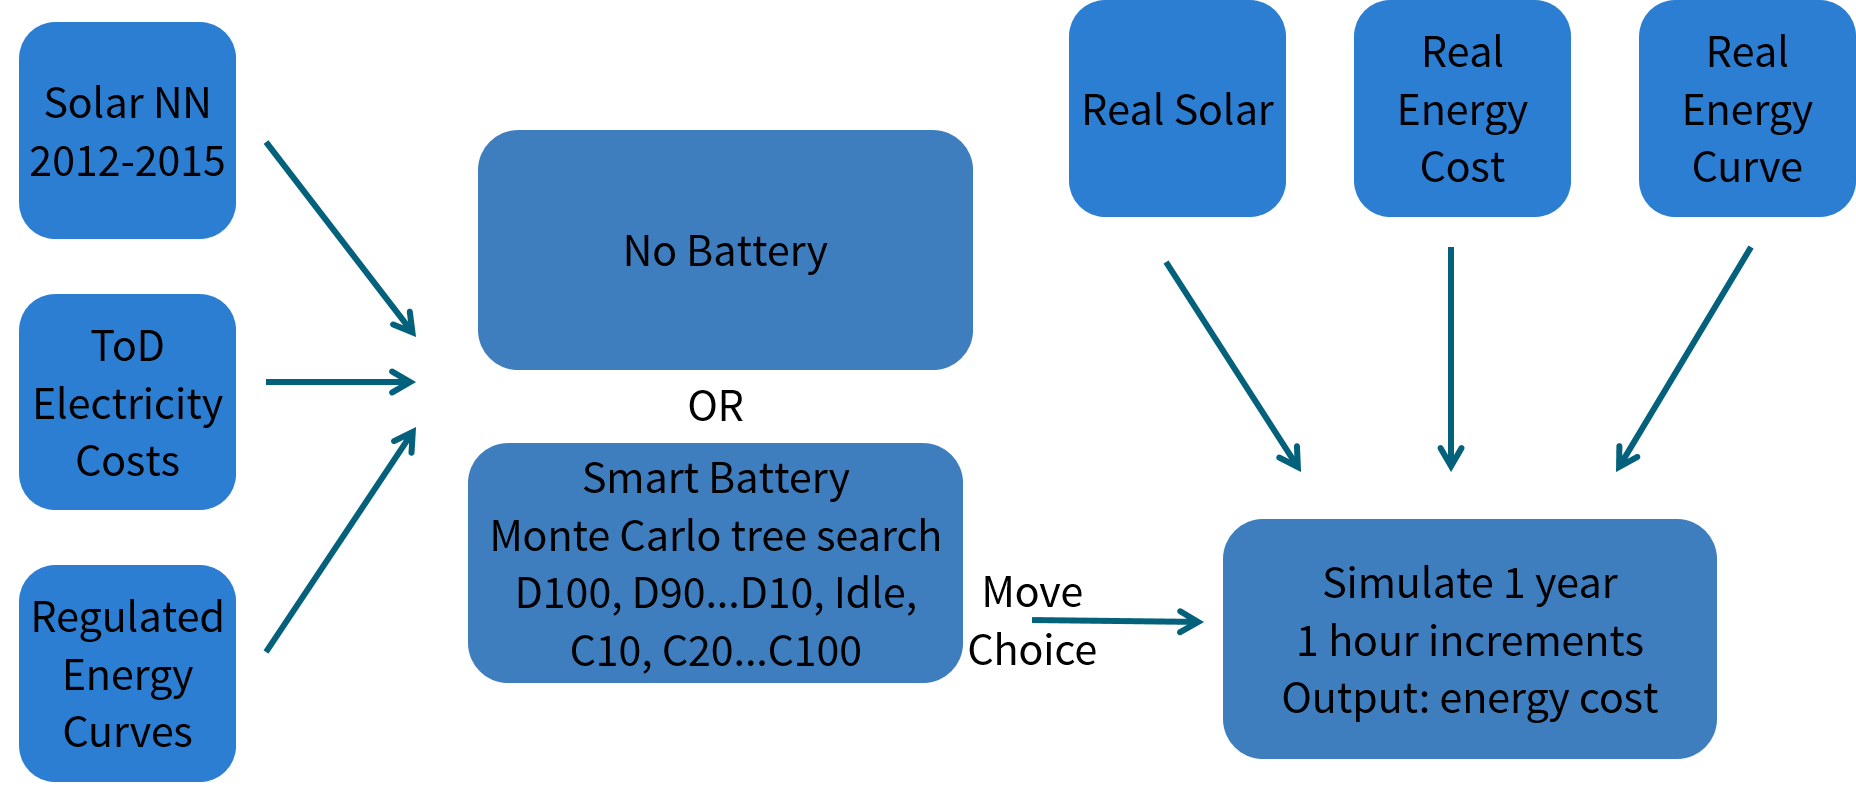
\includegraphics[width=0.50\textwidth]{./figures/image_1.png} \\
   \end{tabular}
   \end{center}
\caption{The layout of the simulation program}
  \vspace{+1mm}
\label{program_layout}
\end{figure}

Figure \ref{program_layout} represents the layout of the simulation program. The bubbles on the left represent \textbf{prediction} components, the boxes in the middle represent the \textbf{decision} components, and the right-side portion represents the \textbf{outcome} components.

\subsection{Prediction: mechanisms to enable other components to make informed decisions}

The simulator allows for several prediction mechanisms.

\begin{itemize}
  \item \textbf{Solar:} Solar prediction is done using a neural network. The actual details of this network are part of a different study. This neural network is trained on information from all of 2012-2015. The inputs for this neural network are time of the day, day of the year, temperature, precipitation, and forecast sky visibility. This information was obtained from several local sources, including Apogee Instruments in Logan Utah, as well as the Logan Utah airport. In getting estimates from the neural network, it was decided to use the actual, measured values of these conditions for 2016 as the predicted values. While this many not be entirely accurate, 24-hour forecasts are accurate enough that it is anticipated the differences will not be drastic. For future studies, some noise could be added to these values to better simulate real conditions.
  \item \textbf{Time-of-day Energy Pricing:} For this paper, time-of-day energy pricing information was obtained from Rocky Mountain power. Rocky Mountain power posts time-of-day pricing that schedules every hour into either off-peak or on-peak pricing. Off-peak pricing yields a discount of \$0.01401 per kWh of energy consumed off-peak, and an additional charge of \$0.04376 per kWh of energy consumed on-peak, per the schdule shown in Figure \ref{tod_pricing} . The base rate was determined \$0.1075 per kWh, taken from an author's monthly energy bill. Thus, given a time of the day, day of the year, and the year, the predictor returns the real cost of energy for that time. The simulator has facilities in place for more robust time-of-day pricing information, such as those proposed for the future updating pricing in 15-minute or other intervals, but these features were not implemented at this time.
  \item \textbf{Home Energy usage:} The home energy predictor is intended to represent two different homes, one a typical home with typical energy-usage habits, and the other a "smart home". A smart home is assumed to contain smart appliances and other enhancements that allow energy usage to be coordinated and scheduled to occur at different times. The goal is that a smart home might have a flatter daily power curve, where electrical loads that might typically occur simultaneously in the evening are intead dispersed more evenly to low-use periods of the day, such as late night and early morning.

  For this paper, two energy curves were obtained from a study conducted by Oracle \cite{fischer_we_2014} where over 800,000 power curves were studied to determine consumer energy usage patterns. It was found that most curves could be lumped into five different categories. The most common was termed the "evening peaker", representing nearly half of all users. The evening peaker does as you might expect and has a peak-load in the evenings that is significantly higher than other loads throughout the day. Another curve, termed the "steady eddy", is nearly flat, with mild increases in usage in the morning and evening. For the purpose of this paper, it was assumed the steady eddy curve is what might be possible with a smart home. Both energy curves are normalized to consume the same total amount of energy over the course of a day. Thus, the curves might not represent a "smart home" in terms of reducing overall energy consumption, but they do allow study of whether shifting loads to off-peak hours is valuable. The actual curves  an be found in Figure \ref{energy_curves}.

  \begin{figure}
   \begin{center}
    \begin{tabular}{cc}
     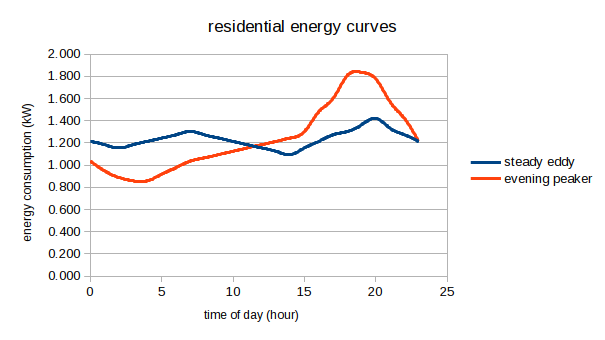
\includegraphics[width=0.50\textwidth]{./figures/energy_curves.png} \\
     \end{tabular}
     \end{center}
  \caption{Energy curves used for this experiment. Both curves represent idential energy usage over 24 hours.}
    \vspace{+1mm}
  \label{energy_curves}
  \end{figure}

  Using the time of day, the home energy usage predictor simply references the power curve of the simulated home to determine power usage for any hour. The simulator is set up to allow for more varied predictions if supplied.
\end{itemize}

\begin{figure}
 \begin{center}
  \begin{tabular}{cc}
   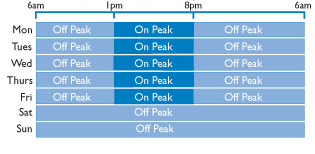
\includegraphics[width=0.50\textwidth]{./figures/utah_tod_pricing.png} \\
   \end{tabular}
   \end{center}
\caption{Time-of-day pricing breakdown for Utah}
  \vspace{+1mm}
\label{tod_pricing}
\end{figure}

\subsection{Decision: uses predictions to estimate costs of available moves and determine which move is best}

The decision component of the simulator has access to all predictors but not the actual values. This was done to represent real conditions as accurately as possible.

The decision process only comes into play when a battery is present. The purpose of the decision process is to look at all the options the battery has at each hour of the day and choose the best option. For this paper, the battery uses the Monte Carlo tree search method. 

Monte Carlo Tree Search involves random sampling of states to completion. It is typically broken down into the following steps \cite{noauthor_monte_2016}:

\begin{enumerate}
  \item \textbf{Selection:} from the starting game state, use some sort of heuristic to choose a next game state to explore
  \item \textbf{Expansion:} from this chosen next game state, randomly choose a further game state to explore
  \item \textbf{Simulation:} randomly choose moves to simulate a game until a win or loss state is encountered
  \item \textbf{Backpropagation:} traverse back to the starting game state, using the simulation results to update corresponding nodes
\end{enumerate}

While there are plenty of papers detailing the use of Monte Carlo tree search for use in perfect information, 2-player games \cite{takeuchi_evaluation_2008} \cite{browne_survey_2012}, there is little research looking at Monte Carlo tree search as a tool in a single player game \cite{schadd_single-player_2012}. However, Monte Carlo tree search seems like a good fit for a battery charging decision algorithm. At every point, there are a contrained number of choices for what a battery can do. The battery has ideas about what might happen in the future, but does not know for sure. In addition, the choices the battery makes now will have an impact on future perfomance. Monte Carlo tree search is a good option that allows a battery to simulate making a decision and then playing out a random simulation to completion. The method includes facilities for determining which pathways to explore. When simulations are complete, the algorithm determines which of all the possible choices puts the battery in the best position in the future.

There were a few details to work out with single player Monte Carlo tree search that are not a problem in typical applications.
\begin{itemize}
    \item Typical Monte Carlo tree search completes a simulation when a game is either won, lost, or drawn. For the simulations in this paper, the simulation will actually complete after a specified number of rounds, such as 24. Each round represents one hour into the future to take into consideration. Once the round limit has been reached, the total cost of all the decisions made to that point is calculated, and that value is used to back propagate through the algorithm.
    \item In a perfect information 2-player game, there is typically a winner and loser. A binary score is thus typically enough for rewarding Monte Carlo tree search simulations. However, in the application in our paper, the reward is instead based on how much electricity a system has to purchase from the energy grid. Thus, the number can be any value starting at 0 (there is also possibility of net metering or earning credits for producing more energy than you consume, which is ignored in this paper). In order for the statistical sampling of the algorithm to work correctly, somehow these unbounded values need to be constrained to something between 0 and 1. Eventually, the equation \(1 - \frac{cost}{cost + 1}\) was settled on. With this equation, the closer a value is to \$0 cost, the closer the reward is to the max value of 1. Likewise, as the cost increases, the reward approaches 0. This equation was adequate for the method to work.
    \item For Monte Carlo tree search to work, there need to be choices of moves to make. "Idle" is always a choice, where the battery chooses to do nothing. However, the battery cannot simply "charge" or "discharge", as there are different rates of both. Thus, it was decided to allow for the battery to charge or discharge at any rate from 10-100\% of the max rate of the battery, in increments of 10\%. This yields 21 possible options for the battery to choose from. The algorithm ensures that options are not available in each round that would overcharge or overdischarge the battery.
\end{itemize}

Once the battery makes a decision on the best action for the next hour, that decision is sent to the outcome portion of the simulator.

\subsection{Outcome: determines the actual cost of a decision}

This final component is fairly basic. The main job of this component is to determine the actual cost of energy at each point in time. If there is no battery present, the system simply looks at how much energy is being consumed by a system, how much energy is entering a system, and how much of that energy had to be purchased from the utility company and at what price. A battery can either be feeding into or pulling from the system, depending on whether it has chosen to charge or discharge for a period of time. The outcome module simply puts all of this together and returns the actual cost of energy for the specific time period in question, and also updates the battery charge state as needed.

Thus, all the parts of the simulator boil down to a few basic inputs of time of day, day of year, and year, and come out as a single number representing cost.

\section{EXPERIMENTS}
In order to complete the experiments, a few assumptions had to be made and are stated here.

\begin{itemize}
  \item The household being simulated was assumed to be "average", which means it uses 10,812 kWh of energy per year \cite{noauthor_how_nodate}. This works out to be just over 29 kWh per day.
  \item The household has a 5 kW solar panel array, which is reportedly the most common solar panel size in the US.
  \item The battery system is a Tesla Powerwall 2, with a 13.5 kWh capacity and a 5 kW max discharge/charge rate. It is also assumed that the battery is "perfect" and thus does not incur any parasitic loss while charging, discharging, or idling.
  \item The smart battery mainly looks 24 hours into the future before making a decision, though tests of 12 and 36 hours were also run.
  \item The home has an identical power curve every day, regardless of the time of year.
  \item The home is not able to take advantage of net metering, where excess energy can be "sold" back into the electrical grid in exchange for energy credits.
\end{itemize}

With this is mind, there were three experiments conducted using the simulator, with the potential for more at a future time.

\begin{itemize}
  \item \textbf{Experiment 1:} Examining yearly energy cost of the 8 possible combinations of technologies
  \item \textbf{Experiment 2:} Looking at the technologies in isolation
  \item \textbf{Experiment 3:} Exploring changes in yearly energy cost of looking ahead 12, 24, and 36 hours before making a decision
\end{itemize}

\subsection*{Experiment 1: Examining yearly energy cost of the 8 possible combinations of technologies}

For this experiment, 8 different simulations were run, each representing a unique combination of the 3 technologies being studied. Those simulations including a battery run 24 hours of predictions before making a decision. A cost is obtained for every hour of the day, and those costs are summed over all of 2016 to obtain the results found in Figure \ref{experiment_1}.

\begin{figure}
 \begin{center}
  \begin{tabular}{cc}
   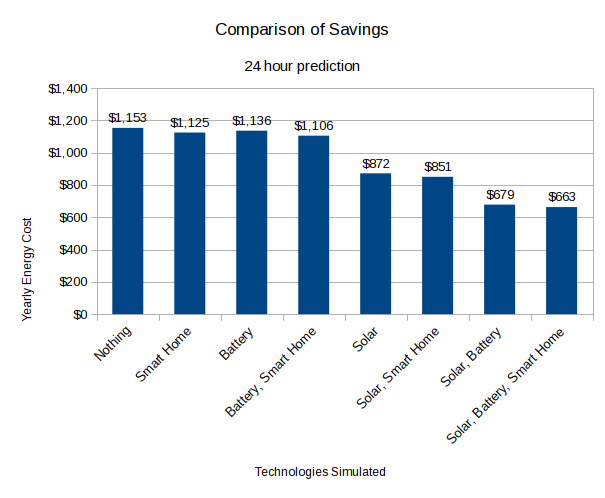
\includegraphics[width=0.50\textwidth]{./figures/experiment_1.png} \\
   \end{tabular}
   \end{center}
\caption{The results of simulating all combinations of technologies for all of year 2016}
  \vspace{+1mm}
\label{experiment_1}
\end{figure}

There are a few things of interest from these results.

First, it would appear that nearly negligible energy savings are to be found without solar. Even the battery, able to take advantage of cheaper energy prices, offers very little financial benefit. Solar immediately contributes 20-25\% savings in cost.

Another point of interest is that once you have solar, the battery becomes significantly more useful, saving an additional 15-20\% in energy costs. Thus, it can be seen that solar and a battery are superadditive, meaning the two technologies together contribute greater savings than the sum of their individual potential savings.

Finally, it would appear that the smart home, as represented in this study as shifting loads to off-peak times, contributes very little, even when coupled with solar and/or a battery.

\subsection*{Experiment 2: Looking at the technologies in isolation}

The next experiment considers each technology in isolation, showing the overall cost of all simulations that include a technology, compared to all simulations that did not include a technology. These results are found in Figure \ref{experiment_2}.

\begin{figure}
 \begin{center}
  \begin{tabular}{cc}
   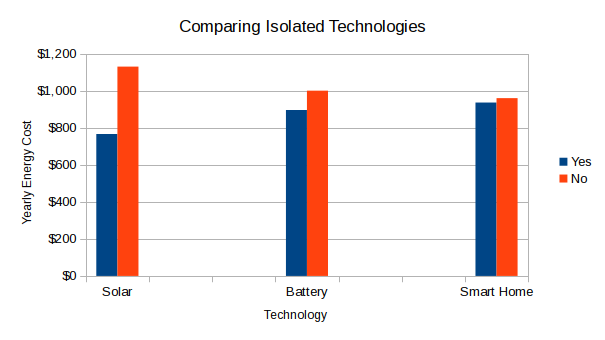
\includegraphics[width=0.50\textwidth]{./figures/experiment_2.png} \\
   \end{tabular}
   \end{center}
\caption{The results of isolating each technology}
  \vspace{+1mm}
\label{experiment_2}
\end{figure}

These results suggest that all technologies do contribute something in energy cost savings. As found in the previous experiment, solar contributes the most, with battery being the next greatest contributor. These results do suggest that smart home technology does contribute some to energy savings, though the contribution is so small as to hardly justify the expense of installing and maintaining such technologies.

\subsection*{Experiment 3: Exploring changes in yearly energy cost of looking ahead 12, 24, and 36 hours before making a decision}

This final experiment focuses more on the algorithm used to make a battery decision. As discussed previously, the Monte Carlo tree search algorithm used in this paper terminates a simulation after a specific number of hours in the future. The previous results used a fixed number of 24 hours in the future. This experiment runs the same simulation for all of year 2016, but terminates a battery simulation at times of 12, 24, and 36 hours in the future. These results are contained in Figure \ref{experiment_3}.

\begin{figure}
 \begin{center}
  \begin{tabular}{cc}
   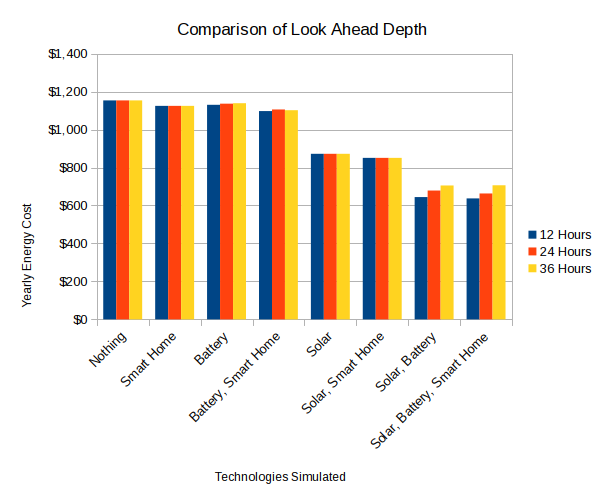
\includegraphics[width=0.50\textwidth]{./figures/experiment_3.png} \\
   \end{tabular}
   \end{center}
\caption{The results of allowing the battery to look 12, 24, and 36 hours into the future before making a decision}
  \vspace{+1mm}
\label{experiment_3}
\end{figure}

Of course the results with no battery are identical. However, when the battery is introduced alongside solar, there can be seen minor reductions in energy costs as simulation depth is reduced. These results are significant because this is a "free" upgrade, meaning it did not require any additional investments in hardware, only a modification to the algorithm running on already present hardware.

There are a few things that might explain these results. If you run the exact same simulation repeatedly, you will find that the battery does not always choose the same action, but instead chooses amongst several similar actions. Thus, in 10 runs of the simulator for the same hour, you might find several "c10", several "c20", and several "idle", meaning the battery chooses to charge at 10\% of the max rate, 20\% of the max rate, or idle. While these differences might be nearly insignificant in the period of 1 hour, over the course of a year the difference between charging at 10\% and 20\% can add up to a meaningful amount. When you run the simulation looking ahead only 12 hours, the algorithm can be more confident in a final decision as there is less variability in the end result. As you increase the search depth, there will be more variability in the end result, which may make deciding what to do now more difficult and prone to error.

Allowing the Monte Carlo tree search algorithm to run more simulations or simulate for a longer time might allow the results of 24 or 36 hour predictions to normalize with those of 12 hour predictions. However, more work would need to be done to understand if looking ahead that far is every advantageous. If you can always obtain results simply as good as 12 hours but not necessarily better, then there is no need to simulate beyond 12 hours. Perhaps simulating less than 12 hours ahead might be even more useful. These are all areas for further study.

\section{CONCLUSION}
There can be several conclusions drawn from the results of this study.

\begin{itemize}
    \item "Free" energy will always beat out "cheap" energy. In this study, solar panels represent "free" energy, whose cost is nothing. While the battery can take advantage of "cheap" energy through time-of-day pricing, the costs savings are so small, roughly \$0.015 per kWh over the normal non time-of-day pricing, that it takes lots of careful maneuvers to experience any real relevant savings, particularly enough to justify investing in an expensive technology.
    \item While a standalone battery might be impractical in the scenario laid out in this simulation, a battery system coupled with solar panels might be worth the investment, depending on the circumstances. This is similar to the results from other studies \cite{truong_economics_2016}.
    \item In the smart home scenario outlined in this paper, where loads are merely shifted rather then reduced, smart home technology does not seem to significantly reduce energy costs. Thus, smart home technologies may be better suited to increase comfort and convenience rather than reduce energy bills. However, smart home technologies exist that can actually reduce overall energy usage. Such technologies may be worth studying in a formal way.
    \item There are many factors that play into this study that could vary drastically from one situation to another. This paper made many assumptions on load, solar panel size, battery size, usage patterns, and pricing. If this study were to be conducted using different information representing a different circumstance, locale, etc, the results might be very different. For instance, in an area with drastic time-of-day differences in pricing, a standalone home battery system might be found to be more relevant. Other areas with reduced solar radiation might show solar panels to be less of an advantage. Different energy usage curves might show smart home technology to be more beneficial than this study showed.
\end{itemize}



\section{FURTHER STUDY}
The results of this paper, as well as areas that were not able to be explored, demonstrate many areas that deserve further research.

\begin{itemize}
    \item A future study could explore different time-of-day pricing scenarios. For example, this study assumed the user took part in Rocky Mountain Power's time-of-day pricing program. However, there is also a traditional program offered that has a flat rate for all times of the day. It may be interesting to explore whether any significant savings can be found using the technologies in this paper when switching from the standard model to the time-of-day mode.
    \item Different locales should be studied to understand the benefits of technologies in different areas. For instance, this study assumed the location as Logan, UT, which has a decent amount of solar radiation. Conducting the same study for somewhere such as Seattle and comparing it to somewhere else such as Phoenix could yield vastly different results that might be worth studying.
    \item This paper took the approach of using Monte Carlo tree search for deciding the battery action at each hour. There are many optimizations that might be made to Monte Carlo tree search that might yield better results. In addition, it might be interesting to try entirely different optimization algorithms. The simulator program is set up to do that if someone in the future chooses to implement such a feature.
    \item It might be beneficial to add more granularity to the battery decisions. This study only allowed 21 possible battery states. However, it might be better to allow for a continuum of states. Such a modification would require different algorithms than Monte Carlo tree search, but might allow for greater savings with no necessary modifications in hardware.
    \item It may be beneficial to explore different energy usage curves. This study assumed an "ideal" curve to be as close to steady as possible. However, it might be even more beneficial to shift loads from on-peak times (such as evenings) to entirely off-peak times, such as the middle of the night or early morning. It would be fairly easy to simulate different curves using the current simulator.
    \item There are other technologies such as wind turbines and heat pumps that are marketed to consumers. Adding these technologies to the system would allow for a more comprehensive look at the state of current technologies.
    \item Some locales allow for "net metering", where excess energy can be fed into the power grid in exchange for energy credits. This simulation assumed that net metering was not permitted. However, the change would be trivial to allow net metering in simulations. This could yield interesting results that may be helpful in exploring areas such as energy policy.
\end{itemize}

\section*{Acknowledgment}

Portions of the software used in this paper was forked from andysalerno/reversi\_ai on GitHub \cite{noauthor_winning_2016}. All forked software was heavily modified for the specific needs of the tests in this paper. To find the software as used in this paper, visit BigOz on GitHub.

Data for this study came from multiple sources. Weather data for Logan, UT was from the Utah Climate Center website. Solar radiation data is courtesy of Apogee Instruments in Logan, UT. Time-of-day pricing information for Utah comes from Rocky Mountain Power. Average home energy usage information comes for the USEIA. Other data sources are credited where appropriate.

\bibliographystyle{plain}
\begin{small}
\bibliography{flourish}
\end{small}
\end{document}